\testCom
{%Номер задачи
	3.111
}
{%Условие
	условие
}
{%Дано
	дано
}
{%Найти
	найти
}
{%Решение
	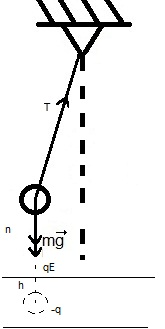
\includegraphics[height=50mm]{3_111.jpg}\\
	$m \der{x}{t}{2} = - mg \frac{g}{h} \Rightarrow \omega_1^2 = \frac{g}{h}$\\
	$\frac{T_2}{T_1} = \frac{1}{\eta} \quad \frac{\omega_2^2}{\omega_1^2} = \eta^2$\\
	с зарядом:	\\
	$m \der{x}{t}{2} = - \left( \frac{q^2}{16 \pi \epsilon_0 h^2}+ mg \right ) \frac{x}{h}$\\
	$\omega_2^2 = \left( \frac{q^2}{16 m \pi \epsilon_0 h^2} + \cancel{mg} \right) \frac{1}{h}$\\
	$\eta^2 = 1 + \frac{q^2}{16 m \pi \epsilon_0 h^2} \cdot \frac{1}{g} \Rightarrow q = 4 h \sqrt{\pi \varepsilon_0 mg (\eta^2 + 1)}$\\
}

